% !TEX program = xelatex
\documentclass[UTF8,11pt,fontset=none]{ctexart}
% Use the TeX-distributed AR PL SungtiL GB TrueType font.
% TrueType embedding avoids external Adobe-GB1 CMap rendering dependencies.
% A bare filename also works inside the editor compiler sandbox.
\setCJKmainfont[Script=Default,AutoFakeBold=2,AutoFakeSlant=0.2]{gbsn00lp.ttf}
\setCJKsansfont[Script=Default,AutoFakeBold=2]{gbsn00lp.ttf}
\setCJKmonofont[Script=Default,AutoFakeBold=2]{gbsn00lp.ttf}
\usepackage[a4paper,margin=2.4cm]{geometry}
\usepackage{amsmath,amssymb,booktabs,array,enumitem,xcolor,tikz,listings}
\usepackage[skins,breakable]{tcolorbox}
\usepackage{needspace}
\usepackage{hyperref}
\definecolor{caramel}{HTML}{A9713C}
\definecolor{rosec}{HTML}{D8678F}
\definecolor{paper}{HTML}{FBF4EA}
\definecolor{inkc}{HTML}{3B2E24}
\hypersetup{colorlinks=true,linkcolor=caramel,urlcolor=rosec,
 pdftitle={体育赛程编制：从图的因子分解到整数规划},pdfauthor={GPT}}
\linespread{1.08}
\setlength{\parskip}{0.25em}
\setlist{itemsep=0.15em,topsep=0.3em}
\newtcolorbox{keybox}[1][小结]{breakable,enhanced,colback=paper,colframe=caramel,
 boxrule=0.7pt,arc=1.5mm,left=3mm,right=3mm,top=2mm,bottom=2mm,
 title={\bfseries #1},coltitle=white,colbacktitle=caramel,fonttitle=\bfseries}
\newtcolorbox{warnbox}[1][注意]{breakable,enhanced,colback=rosec!6,colframe=rosec,
 boxrule=0.7pt,arc=1.5mm,left=3mm,right=3mm,top=2mm,bottom=2mm,
 title={\bfseries #1},coltitle=white,colbacktitle=rosec,fonttitle=\bfseries}
\lstset{language=Python,basicstyle=\ttfamily\footnotesize,
 keywordstyle=\color{caramel}\bfseries,commentstyle=\color{inkc!65},
 stringstyle=\color{rosec},breaklines=true,columns=fullflexible,
 keepspaces=true,showstringspaces=false,frame=single,rulecolor=\color{caramel!50},
 backgroundcolor=\color{paper},aboveskip=0.8em,belowskip=0.8em}
\title{\bfseries 体育赛程编制\\[0.35em]
\large 从“大家都要交手一次”到图的因子分解与整数规划}
\author{数学建模笔记}
\date{2026 年 10 月}
\begin{document}
\maketitle\pagestyle{plain}\thispagestyle{empty}
\begin{keybox}[这篇文章想做的事]
班级篮球赛有六支队伍，每两队都要交手一次，同一轮谁也不能分身打两场。
最少要安排几轮？如果某天场地不能用，还有两场比赛都希望压轴，又该怎么办？

这篇文章从一张可以手工检查的赛程表出发，慢慢认识图、匹配、1-因子和因子分解，
再把规则翻译成整数规划。\textbf{不需要预先学过图论或优化}：
每个符号都会先用比赛解释。我们也会区分“排得下”“轮数最少”和“尽量让大家满意”，
因为它们是三个不同的问题。（本文由 GPT 写作）
\end{keybox}

\section{先说清楚：我们在排什么比赛}
六支队伍记作 A、B、C、D、E、F。先考虑最简单的\textbf{单循环赛}：
每两支不同队伍恰好交手一次，不区分主客场。
这里的“一轮”是一段预先划好的比赛时间，每支队伍在这一轮最多打一场。
先假设每轮有三块场地，能够同时举办三场比赛，且各场比赛占用相同长度的时段。

不要把“六队循环赛”与淘汰赛混在一起：循环赛不会因为输球就少一个对手。
也暂时不安排具体开球分钟、裁判和休息天数；这些都是后面可以再加的条件。

\subsection{一共多少场，至少多少轮}
A 要和另外五队交手，六支队伍各数一遍得到 $6\times5$；
但 A 对 B 被 A、B 各数了一次，所以总比赛数是
\[
\frac{6\times5}{2}=15.
\]
每队每轮最多打一场，而每队要打五场，至少需要五轮。
从场地看也一样：每轮最多三场，十五场至少要 $15/3=5$ 轮。

\begin{warnbox}[下界是“不能更少”，还不是“排得出来”]
数出来“五轮以下不行”，只完成了证明的一半。
要说五轮最优，还必须真的给出一张不重赛、不漏赛、没人分身的五轮表。
\end{warnbox}

\Needspace{10\baselineskip}
\section{把比赛画成一张图}
这里的\textbf{图}不是统计图表，而是一种只关心“谁和谁有联系”的数学对象：
\begin{itemize}
\item 一个\textbf{顶点}代表一支队伍；
\item 一条\textbf{边}连接两支队伍，代表它们之间的一场比赛；
\item 某个顶点连着几条边，就说它的\textbf{度}是多少，表示该队总共要打几场。
\end{itemize}
两队都要交手，所以任意两个不同顶点之间都有一条边。
这样的图叫\textbf{完全图}；六个顶点的完全图记作 $K_6$。
字母 $K$ 只是约定的记号，不需要从中读出别的意思。

\begin{center}
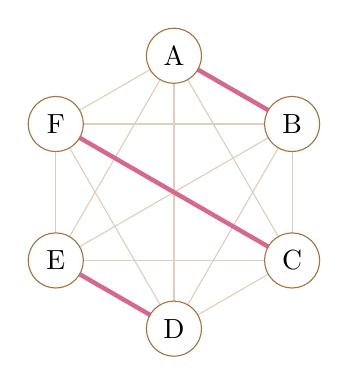
\begin{tikzpicture}[scale=1.05]
\foreach \i/\name in {0/A,1/B,2/C,3/D,4/E,5/F}
 {\coordinate (v\i) at (90-60*\i:1.65);}
\foreach \i in {0,...,4} {\pgfmathtruncatemacro{\start}{\i+1}
 \foreach \j in {\start,...,5} {\draw[caramel!35] (v\i)--(v\j);}}
\foreach \i/\j in {0/1,2/5,3/4} {\draw[rosec,line width=1.6pt] (v\i)--(v\j);}
\foreach \i/\name in {0/A,1/B,2/C,3/D,4/E,5/F}
 {\node[circle,draw=caramel,fill=white,minimum size=7mm] at (v\i) {\name};}
\end{tikzpicture}

\small 灰褐色边表示全部十五场比赛；粉色的三条边表示第一轮。
\end{center}
边交叉不表示多打一场，图上也没有“交叉处的队伍”；只有标了字母的点才是队伍。
这一点初次看图时很容易误读。

\section{一轮比赛，为什么叫一个 1-因子}
\subsection{先认识匹配}
假如把 A--B 和 A--C 同时放进一轮，A 就要分身。
在图里，这是两条边共用了顶点 A。
所以一轮能够一起举行的比赛，必须是\textbf{互不共用顶点的一组边}，叫\textbf{匹配}。
例如 A--B、C--F 可以同轮进行，但 D、E 还在休息。

若六支队伍每支都恰好出现一次，这个匹配就叫\textbf{完美匹配}。
例如 A--B、C--F、D--E。它包含三个比赛，也恰好覆盖六支队伍。

\subsection{再拆开“1-因子”这个词}
图论里的\textbf{因子}，指保留原图全部顶点、选取一部分边得到的子图。
若在这个子图中，每个顶点的度都等于 $1$，它就叫\textbf{1-因子}。
因此，\textbf{完美匹配选出的边，连同全部顶点，就是一个 1-因子}。

这里的“1”是每支队伍在这一轮\emph{恰好打一场}，不是“第一轮”。
第五轮如果人人出场，也同样是一个 1-因子。

\begin{keybox}[赛程语言与图论语言的字典]
\begin{center}
\begin{tabular}{ll}
\toprule
比赛里说的话 & 图论里说的话\\\midrule
队伍 & 顶点\\
两队之间的一场比赛 & 边\\
一轮没人打两场 & 这一轮的边构成匹配\\
一轮所有队伍都打一场 & 这一轮构成完美匹配，即一个 1-因子\\
每场恰好安排到某一轮 & 把全部边分成互不重叠的若干组\\\bottomrule
\end{tabular}
\end{center}
这里“不重叠”说的是\textbf{边不重复}。各轮仍然使用同一批队伍，也就是同一批顶点。
\end{keybox}

\section{整张五轮表，就是一次因子分解}
下面这张表可以逐行检查，也可以逐队检查：
\begin{center}
\begin{tabular}{cccc}
\toprule
轮次 & 第 1 场 & 第 2 场 & 第 3 场\\\midrule
1 & A--B & C--F & D--E\\
2 & A--C & B--D & E--F\\
3 & A--D & C--E & B--F\\
4 & A--E & D--F & B--C\\
5 & A--F & B--E & C--D\\\bottomrule
\end{tabular}
\end{center}
每一行是一个 1-因子；五行合起来，每条边恰好出现一次。
这就叫 $K_6$ 的一个\textbf{1-因子分解}。

若把各轮的边集合分别记为 $F_1,\dots,F_5$，把全部边记为 $E$，可以简写为
\[
E=F_1\mathbin{\dot\cup}F_2\mathbin{\dot\cup}\cdots\mathbin{\dot\cup}F_5.
\]
符号 $\dot\cup$ 的意思是“合在一起，并且彼此没有重复元素”。
它不是把六个顶点拆开，也不是把某个数字做乘法分解。

换一种说法：给每轮选一种颜色，把该轮比赛的边涂成这个颜色。
同一顶点上不能出现两条同色边。这也叫\textbf{边着色}。
在我们的五轮最紧凑赛程里，每种颜色恰好构成一个 1-因子。

\section{不靠试凑：怎样系统地造出赛程}
\subsection{六队的做法：固定一队，另外五队轮流转}
固定 A，把另外五队编成一圈编号
\[
\text{B}=0,\quad\text{C}=1,\quad\text{D}=2,\quad\text{E}=3,\quad\text{F}=4.
\]
编号按钟面循环，$4$ 再向前走一格回到 $0$，$0$ 向后走一格回到 $4$。
第 $t$ 步让 A 对编号 $t$ 的队，其余队伍按
\[
(t+1,\ t-1),\qquad(t+2,\ t-2)
\]
配对，超出 $0$ 到 $4$ 的范围就沿圈绕回去。让 $t$ 依次取 $0,1,2,3,4$。

例如 $t=0$ 时，A 对 B；$1$ 与 $-1$ 配对，其中 $-1$ 绕回 $4$，所以是 C 对 F；
$2$ 与 $-2$ 配对，其中 $-2$ 绕回 $3$，所以是 D 对 E。
$t=1$ 时则是 A 对 C、D 对 B、E 对 F。上节的五轮表正是这样生成的。
这种循环配对构造通常称作\textbf{圆圈法}的一种写法。

\subsection{一般偶数支队伍：公式只是同一个动作}
设队伍数为 $n=2m$，也就是说 $n$ 是偶数，$m$ 是它的一半。
固定一队记为 $\infty$（只是名字，不表示真的有无限多队），
其余队编号为 $0,1,\dots,q-1$，其中 $q=n-1=2m-1$ 是奇数。
第 $t$ 轮的配对是
\[
F_t=\{\{\infty,t\}\}\ \cup\
\bigl\{\{t+i,t-i\}:i=1,\dots,m-1\bigr\},
\qquad t=0,\dots,q-1.
\]
所有有限编号都按长度为 $q$ 的圈循环。
这里的 $t$ 从 $0$ 开始编号，所以公式中的第 $0$ 轮就是表中的第 $1$ 轮。

\begin{keybox}[为什么它真的不漏、不重]
\textbf{每轮覆盖所有队伍。}除固定队与 $t$ 配对外，
其余编号可写成 $t\pm1,\dots,t\pm(m-1)$，恰好覆盖剩下的 $2m-2$ 支队伍。

\textbf{固定队不会重赛。}它依次遇到每个有限编号一次。

\textbf{其余任意两队也只见面一次。}设编号为 $a,b$。
它们被配成一对时，两个编号加起来一定是 $2t$（允许绕圈）。
在奇数长度的圈上，“乘 $2$”会把全部编号重新排列一遍，因此恰有一个 $t$
满足这个条件。又因为 $a\ne b$，它们分处 $t$ 两侧某个非零距离，
正是公式里列出的某一对。
\end{keybox}
如果想把最后一步写得严格些：若 $2t$ 与 $2u$ 绕圈后相同，
则奇数 $q$ 整除 $2(t-u)$，也就整除 $t-u$；
在 $0,\dots,q-1$ 中只能有 $t=u$。有限集合中的单射也就是双射。
这段证明可以跳过；记住“每对队伍在圈上有唯一的配对时刻”就够了。

因此\textbf{任意偶数支队伍的单循环赛，都能在 $n-1$ 轮内完成}，
并且达到前面数出来的下界。我们既有“不可能更少”的计数，也有“确实做得到”的构造。

\section{如果有奇数支队伍呢}
以五队为例，每队要打四场，但四轮真的够吗？
每轮最多安排两场，总共却有 $5\times4/2=10$ 场，
四轮最多只能放八场。因此\textbf{至少五轮}。

解决办法是添加一支虚拟队伍 $\star$，把五队变六队，照样做 1-因子分解。
谁在某一轮对上 $\star$，谁就在那一轮\textbf{轮空}，虚拟比赛不真的举行。
六队的五轮表中，每支真实队恰好遇到虚拟队一次，所以各轮空一次。

一般地，奇数 $n\ge3$ 时，至少需要
\[
\frac{n(n-1)/2}{(n-1)/2}=n
\]
轮；加虚拟队得到的 $n$ 轮表恰好达到它。
删掉虚拟队之后，每轮是覆盖除轮空队以外所有队的匹配，
\textbf{不是原来奇数个顶点上的 1-因子}，因为奇数个人无法两两配完。

\section{现实条件一加进来，圆圈法就不够了}
基础配对构造并不处理以下要求：
某轮某队不能参赛、某场比赛指定日期、每轮只有两块场地、两场焦点战都想压轴。

例如六队仍有十五场比赛，如果每轮场地只能容纳两场，就至少要
\[
\left\lceil\frac{15}{2}\right\rceil=8
\]
轮。尖括号 $\lceil\ \rceil$ 表示向上取整：七轮只能容纳十四场，只好再加一轮。
这里\textbf{八轮只是新的下界}，具体附加限制下还要检查能否实现。

若 A 在第一轮完全不能参赛，而赛程仍只给五轮，即使场地足够也无解：
A 剩下四轮，却要打五场。不能要求求解器把逻辑上矛盾的条件“优化好”。

\begin{warnbox}[一轮与一块场地不是一回事]
前面的“每轮三场”假设三场能并行。若只有一块场地，
却允许把同一轮的三场依次放在整个下午，必须重新说明一轮有多长、最多装几场。
若还要精确计算休息时间，就应该直接用开球时段建模。
模型里的时间单位要先讲清楚，不能一会儿表示一小时，一会儿表示一天。
\end{warnbox}

\section{整数规划：把“哪场放哪轮”变成开关}
\subsection{变量与两组基本约束}
给队伍编号 $1,\dots,n$，预留 $T$ 轮。
对每对队伍只使用 $i<j$ 的编号，避免 A--B 与 B--A 被当成两场不同比赛。
定义
\[
x_{ijt}=\begin{cases}
1,&\text{队 $i$ 与队 $j$ 在第 $t$ 轮交手},\\
0,&\text{否则}.
\end{cases}
\]
每个变量只能开或关；所谓\textbf{0--1 整数规划}，就是用线性的约束和目标函数组织这些开关。
“线性”表示变量只乘已知常数，不把两个未知开关相乘。

\textbf{每对恰好交手一次：}
\begin{equation}\label{eq:pair}
\sum_{t=1}^{T}x_{ijt}=1\qquad(1\le i<j\le n).
\end{equation}
固定一对队伍，沿时间把开关加起来，要求恰好亮一次。

\textbf{每队每轮最多打一场：}
\begin{equation}\label{eq:team}
\sum_{j<i}x_{jit}+\sum_{j>i}x_{ijt}\le1
\qquad(i=1,\dots,n;\ t=1,\dots,T).
\end{equation}
因为始终把小编号写在前面，找队 $i$ 参与的比赛时要分两段相加。
例如 A 编号最小，就只有第二段；F 编号最大，就只有第一段。
不等号允许轮空，不能在任意 $T$ 下都强迫人人每轮打一场。

六队五轮时，有 $15\times5=75$ 个开关，
基本约束是 $15$ 条“每对一次”与 $6\times5=30$ 条“每队每轮最多一次”，共 $45$ 条。
若没有别的偏好，目标函数写 $\min 0$ 就行：先找一张合法表。

\subsection{图的因子分解怎样藏在方程里}
对偶数 $n$，若恰好取 $T=n-1$，
每队必须在 $n-1$ 轮里完成 $n-1$ 场，所以式 \eqref{eq:team} 必定每轮都取等号。
于是每一轮选中的边都是完美匹配；式 \eqref{eq:pair} 又保证所有边恰好分完。
\textbf{这就是用另一种语言寻找 1-因子分解。}

如果预留更多轮，式 \eqref{eq:team} 可能严格小于 $1$，一轮就未必是 1-因子。
这时模型仍然合法，只是允许有空闲队伍。

\subsection{把现实限制写进去}
每轮最多安排 $C_t$ 场，就加
\[
\sum_{i<j}x_{ijt}\le C_t\qquad(t=1,\dots,T).
\]
某场比赛某轮不能打，直接令相应 $x_{ijt}=0$；
若指定必须打，就令它等于 $1$。
若整支队伍 $i$ 某轮缺席，就把式 \eqref{eq:team} 的右边从 $1$ 改为 $0$。
每条新增约束都应该能反过来读成一句明确的人话。

\Needspace{10\baselineskip}
\section{硬要求和软愿望：六队例子的完整计算}
仍预留五轮，每轮最多三场。另有三条\textbf{硬要求}：
\begin{enumerate}
\item A--B 不能放第一轮；
\item C--D 不能放第五轮；
\item A--F 必须在第三轮举行。
\end{enumerate}
再加两条\textbf{软愿望}：A--B 希望放最后一轮，A--C 也希望放最后一轮。
两场共享 A，所以不可能都如愿。若把两条都写成硬约束，整个模型就无解。

可以改成：每个没实现的愿望罚 $1$ 分，让总罚分尽量小：
\[
\min P=\sum_{t=1}^4x_{\mathrm{AB},t}
       +\sum_{t=1}^4x_{\mathrm{AC},t}.
\]
这里 $x_{\mathrm{AB},t}$ 是 A、B 对应变量的易读写法。
某场只会安排一次，因此它放到前四轮就贡献 $1$，放最后一轮则贡献 $0$。
目标函数仍是线性的。

下面是一张满足全部硬要求、总罚分为 $1$ 的表：
\begin{center}
\begin{tabular}{cccc}
\toprule
轮次 & 第 1 场 & 第 2 场 & 第 3 场\\\midrule
1 & A--D & B--C & E--F\\
2 & A--C & B--F & D--E\\
3 & A--F & B--E & C--D\\
4 & A--E & B--D & C--F\\
5 & A--B & C--E & D--F\\
\bottomrule
\end{tabular}
\end{center}
罚分不可能低于 $1$，因为 A 在最后一轮不能同时对 B 和 C。
表里又确实做到 $1$，所以它就是这个例子的\textbf{最优解}。
最优并不代表只有这一张表，其他轮次与对手组合也可能达到相同罚分。

若某个愿望比另一个重要，可以给它乘不同权重。
但权重表达的是组织者的取舍，不能把“罚分最少”直接叫作\emph{所有意义上的最公平}。

\section{再多考虑一层：主客场与双循环}
\subsection{比赛有方向之后}
此前 A--B 没有方向。若比赛必须安排在其中一队的主场，
改用 $z_{ijt}=1$ 表示“第 $t$ 轮队 $i$ 在主场迎战队 $j$”，其中 $i\ne j$。
现在 $z_{ijt}$ 与 $z_{jit}$ 是两种不同安排。

单循环的“每对一次”变成
\[
\sum_t(z_{ijt}+z_{jit})=1\qquad(i<j),
\]
每队每轮最多一次则是
\[
\sum_{j\ne i}(z_{ijt}+z_{jit})\le1.
\]
定义 $h_{it}=\sum_{j\ne i}z_{ijt}$，表示队 $i$ 本轮是否在主场。
在六队五轮、人人每轮出场的前提下，让每队总主场数为两场或三场，可以写
\[
2\le\sum_{t=1}^5h_{it}\le3.
\]
各队都打五场，不可能人人主客场数完全相等；相差至多一场才是这里合理的平衡要求。

\subsection{限制连续主客场，要说清楚“连续”的含义}
在\textbf{每队每轮都参赛}的条件下，禁止连续三轮全是主场或全是客场，可以写
\[
1\le h_{it}+h_{i,t+1}+h_{i,t+2}\le2
\qquad(t=1,\dots,T-2).
\]
上界排除三个 $1$，下界排除三个 $0$。
若允许轮空，$h=0$ 还可能表示“没比赛”，便不能直接把它当成客场。
需要另设出场变量，并区分“连续三个日历轮次”与“连续三次实际出场”。
这里展示的是扩展的建模方法；附录程序只求前面的无主客场六队例子。

双循环要求每对打两场、各自主场一次，可对每个有序对规定
$\sum_t z_{ijt}=1$。把单循环复制一遍并反转主客场，
就能得到基础双循环表；但这不自动保证日期、旅行、连续客场等附加限制都满足。

\section{怎样使用这两种方法}
条件简单时，圆圈法直接给出达到最少轮数的构造，便于解释，也便于人工检查。
条件复杂时，整数规划可以同时改变配对与轮次，搜索满足限制的赛程。
还可以先用圆圈法提出候选方案，再检查或改进。

\begin{warnbox}[固定一张基础表，可能把答案锁没了]
只允许把某一张圆圈法表的整轮调换顺序，搜索范围比完整整数规划小得多。
若这个范围里找不到满足要求的表，不能据此断言整个排程问题无解。
另一方面，求解器超时也不等于证明无解；只有明确的不可行结论才能这样说。
\end{warnbox}
整数规划也不是把所有现实目标放进去就立刻得到唯一答案：
赛季旅行距离需要描述相邻轮次的所在地，休息公平需要定义休息时长，
这些都超出了“每对打一场”的基础模型。\textbf{规则说清楚，优化才有对象。}

\begin{keybox}[读完之后，应该带走什么]
\begin{enumerate}
\item 把队伍变成顶点、比赛变成边，循环赛就是完全图上的排程。
\item 一轮人人恰好出场，是一个 1-因子；全部比赛按轮分开，是 1-因子分解。
\item 偶数 $n$ 队最少 $n-1$ 轮，奇数 $n\ge3$ 队最少 $n$ 轮；
圆圈法和虚拟队不仅猜出数字，还给出了能达到它的构造。
\item 整数规划用“比赛--轮次”开关表达同一个问题，能继续加入日期、场地与主客场限制。
\item 硬要求决定能不能排，软目标决定更喜欢哪张表。最少轮数、最小罚分与公平评价要分别说。
\end{enumerate}
\end{keybox}

\begin{keybox}[参考与继续阅读]
\begin{itemize}
\item R.~V.~Rasmussen, M.~A.~Trick，
\href{https://data.math.au.dk/publications/wp/2006/imf-wp-2006-02.pdf}{Round robin scheduling: a survey}，
Aarhus University 工作论文（2006）。可进一步了解体育排程的术语、主客场模式与优化问题。
\item \href{https://docs.scipy.org/doc/scipy/reference/generated/scipy.optimize.milp.html}{SciPy 官方 milp 文档}。
附录使用其整数性、变量界与线性约束接口，SciPy 至少需要 $1.9$。
\end{itemize}
\end{keybox}

\appendix
\section{可以运行的六队例子}
附带文件 \texttt{赛程示例.py} 同时包含圆圈法与整数规划。
安装 NumPy、SciPy 后执行 \texttt{python3 赛程示例.py}，会打印五轮表和总罚分。
不同求解器版本可能返回不同但同样最优的表；应检查规则与罚分，而不是要求每一行都相同。
下面节选求解器调用与结果校验；其中的代价向量、变量界和约束矩阵由完整文件前半段构造。
这段节选依赖前面的变量，请运行完整文件，而不是只复制本页代码。
代码中队伍 A 到 F 编号为 $0$ 到 $5$，轮次也从 $0$ 开始，第三轮写作 $t=2$。
\begin{lstlisting}
result = milp(cost, integrality=np.ones(len(candidates)),
              bounds=Bounds(lo, hi),
              constraints=LinearConstraint(A.tocsc(), lower, upper),
              options={"mip_rel_gap": 0})
if result.status != 0:
    raise RuntimeError(result.message)
bits = np.rint(result.x)
assert np.max(np.abs(bits-result.x)) < 1e-6
assert np.all(bits >= lo) and np.all(bits <= hi)
values = A @ bits
assert np.all(values >= np.array(lower)-1e-6)
assert np.all(values <= np.array(upper)+1e-6)
selected = [g for g, x in zip(candidates, bits) if x == 1]
schedule = [[(i, j) for i, j, s in selected if s == t]
            for t in range(T)]
return schedule, int(round(result.fun))
\end{lstlisting}
\end{document}
